\documentclass[a4paper, 12pt]{scrartcl}

\usepackage[utf8]{inputenc}
\usepackage[english, ngerman]{babel}
\usepackage[T1]{fontenc}
\usepackage{amsmath}
%für Bilder
\usepackage{graphicx}
%deutsche anführungszeichen
\usepackage{csquotes}\MakeOuterQuote{"}
%ränder
\usepackage[left=3cm, right=4cm, top=3cm, bottom=2.5cm]{geometry}
\usepackage[numbers, round]{natbib}
%spacing
\usepackage[onehalfspacing]{setspace}
%Abkürzungsverzeichnis
\usepackage[printonlyused]{acronym}
%Anzeigen der restlichen Verzeichnisse
\usepackage{tocbibind}
%Literaturverzeichnis
\bibliographystyle{alphadin}

\hyphenation{Schleu-sing-en}

\title{Seminarfacharbeit}
\author{Toni Hausdörfer, Fabian Beez}
\date{27. Mai 2020}

\begin{document}
    
    \maketitle \newpage
    \tableofcontents \newpage
    \input{exports/Abkürzungsverzeichnis.tex} \newpage

    \section{Einleitung}
        %?: mode beetz, ..., in schleusingen schließen immer mehr läden und es werden kaum neue eröffent(abgesehen von restoraunnts). gleichzeitig wird der onlineeinkauf immer attraktiver



Onlinehandel spielt eine immer größer werdende Rolle im Leben von Menschen fast aller Altersschichten. Aufgrund des allmählichen Verschwindens von Geschäften im Gebiet um Schleusingen haben wir uns die Frage gestellt, welche Rolle der Verkauf von Waren über das Internet in unserem Landkreis spielt, und ob die Schließungen einiger Geschäfte auf den Rückgang der Nachfrage für lokale Einzelhändler zurückzuführen ist.

Im Rahmen unserer Arbeit werden wir das Zutreffen folgender Thesen einschätzen:
\begin{itemize}
    \item Der Onlinehandel führt zu einem allmählichen Aussterben von stationären Händlern im ländlichen Bereich.
    
    \item Es gibt Waren, die nicht/kaum online gekauft werden.

    \item Der Onlinehandel schafft weniger Arbeitsplätze als indirekt verringert werden.
\end{itemize}

Außerdem werden wir auf Basis unserer Ergebnisse ein Konzept entwickeln, wie die Nachfrage und der Verkauf von Waren in unserem Landkreis erhöht werden kann.

        \newpage
    
    \section{Historie}
        \subsection{Entstehung}
        \subsection{Entwicklung mit Blick auf Großfirmen wie PayPal}
        \subsection{Beeinflussung der Sozialstrukturen}
        
    \section{PayPal}
        \subsection{Entstehung und grobe Funktionsweise}
        \subsection{Entwicklung}
        \subsection{Einfluss auf die Gesellschaft}
        
    \section{Konsumverhalten}
        \subsection{Veränderungen im Konsumverhalten über die Zeit}
            \iffalse
Einteilung in: Online-Marktplätze + Online-Händler, Intermediäre, Kataloversender, stationäre Händler, Hersteller/Marken \cite{Graf}

entwicklung des kaufprozesses: graf:abbildung; 


änderung kaufablauf: \cite{Schaefers}
\fi

            
        \subsection{Einfluss des Onlinehandels}% Überschneidung mit 7.2
            \input{exports/Fabian/Konsumverhalten-EinflussDesOnlinehandels.tex}
            
        \subsection{Mögliche Probleme und Folgen}
            \input{exports/Fabian/Konsumverhalten-ProblemeUndFolgen.tex}
            
        
    \section{Auswirkungen des Oninehandels auf die Infrastruktur}
        \subsection{Vergangene Änderungen und Entwicklungen}
            \input{exports/Fabian/Infrastruktur-Vergangenheit.tex}
            
        \subsection{Mögliche Entwicklungen in der Zukunft}
            \input{exports/Fabian/Infrastruktur-Zukunft.tex}
            
        \subsection{Probleme mit dem Einfluss des Onlinehandles}
            \input{exports/Fabian/Infrastruktur-Probleme.tex}
            
        
    \section{Globaler Vergleich des Einflusses und der Entwicklung des Onlinehandels}
            \iffalse

deu: 14-tage rückgabe durch §355 BGB

\fi

            
    
    \section{Onlineversandhändeler am Beispiel Amazon} 
         Amazon ist ein Onlineversandhändler, der eine breite Bekanntheit genießt und vor allem im europäischen Raum im Bereich des Onlinehandels einen großen Anteil ausmacht. Während Aliexpress in Asien und östlichen Teilen Europas und Ebay im Norden der EU stark vertreten sind, ist Amazon in Zentral-, Nord- und Westeuropa die Plattform mit dem größten Wert von Verkäufen\cite[S. 22]{EuroCommerce}. Außerdem macht Amazon bereits seit Ende 2017 mehr als die Hälfte der Verkäufe durch Drittanbieter aus\cite[S. 25]{Haendlerbund}. Dementsprechend werde ich in den folgenden Unterpunkten die Firma in Bezug auf ihre Entwicklung, die Auswirkungen dieser und der Konkurrenzfähigkeit zu lokalen Händlern analysieren und auf Basis der Erkentnisse Schlussfolgerungen im Bezug auf Schleusingen und des hildburghäuser Landkreis schließen.

        \subsection{Entstehung und Entwicklung}
            Als Amazon, anfangs noch \emph{cadabra.com}, am 5. Juli 1994 von Jeff Bezos und seiner Frau McKenzie gegründet wurde, hatte wahrscheinlich niemand die Vision eines marktführendem Online-Unternehmens im Kopf - im Gegensatz, Amazon war ursprünglich ein Online-Buchhandel für bestimmte, seltene Bücher\cite[S. 17]{Graf}. Trotz der kleinen Zielgruppe wuchs das Unternehmen in den folgenden Jahren bedeutend: schon zwei Jahre später wurden Aktien angeboten, außerdem wurde anfangs noch fast der komplette Gewinn reinvestiert\cite{Rosoff}, was das Aufkaufen ganzer Unternehmen schon 4 Jahre nach der Gründung ermöglichte, bespielsweise von \emph{pets.com} und \emph{overstock.com}\cite{ChannelAdvisor}. An der Strategie, Unternehmen komplett zu kaufen, hat sich bis heute nichts geändert - im Gegenteil, Amazon kauft heute mehr und größere Unternehmen als je zuvor\cite[S. 27]{Haendlerbund}, wie Audible, Kiva Systems oder Twitch\cite{Sherman}. Der Gewinn wird jedoch nicht mehr ausschließich reinvestiert\cite{Rosoff}. Mit der Zeit expandierte die Firma in viele weitere Gebiete: Cloud Computing mit \ac{AWS} 2002 sowie Musik mit einem Online-Musik-Store und Lebensmittel mit AmazonFresh im Jahr 2007\cite{Sherman, ChannelAdvisor}. Auch bezüglich des Onlinehandels breitete Amazon ab 2000 nach und nach die Produktauswahl aus, wodurch sich der darmalige Buchhandel zu dem heutigen Onlineversandhandel für fast alle Produktereiche entwickelte. Ein wichtiger Schritt zu diesem Ziel war das Ermöglichen von Drittanbieter-Verkäufen ab dem 30. September 1999, was die Bekanntheit und Anzahl der Verkäufe erheblich steigerte\cite{Sherman}. Außerdem wurden weitere Technologien wie Amazon Prime und AmazonBasics entwickelt, die den Onlinehandel und -versand unterstützen\cite{ChannelAdvisor}, aber auch alleinstehende Projekte, wie Kindles, das Fire Phone oder Smart-Home-Geräte\cite{Sherman}.

Die derzeitige Strategie bezüglich des Oninehandels beschrieb Bezos, als "Virtuos Cycle" betitelt, schon 2001  mit folgender Zeichnung\cite{zentail}:
%IST NICHT IMMER DA WO ES SOLL WENN ES ZB NICHT AUF DIE SEITE PASST
\begin{figure}[h]
    \begin{center}
        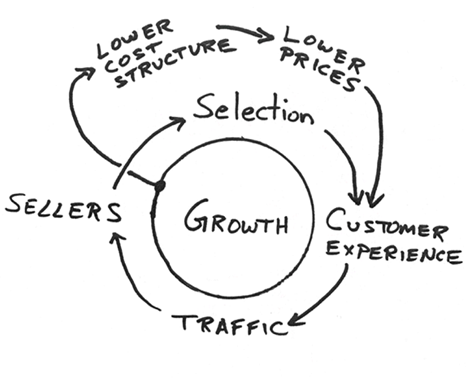
\includegraphics[width=8cm]{media/Fabian-vicious-cycle.png}
        \caption{Amazon's Vicious Cycle}
        \label{vicious-cycle}
        \bildquelle Jeff Bezos, September 2001 %Learn from the Bezos Virtuous Cycle: Leverage and Invest in Infrastructure, www.zentail.com, abgerufen August 2020% https://tinyurl.com/yyu2zz29 DATUM???
    \end{center}
\end{figure} 

Dabei schafft breit gefächerte Produktsegment(Selection) eine positive Kundenerfahrung(Customer Experience), die weitere Verkäufe und Verbreitung durch z. B. Empfehlungen(Traffic) hervorruft. Durch diese hohe Kundenanzahl ist die Plattform wiederrum attraktiver für Drittanbieter und Herstellern(Sellers), die weitere Produkte anbieten und das Produktsegment erweitern. Dieser Teil ist an sich nicht wirklich außergewöhnlich, da viele andere Onlineanbieter eine ähnliche Strategie verfolgen. Jedoch hebt sich Amazon damit ab, ungewöhnlich hohe Summen zu investieren, um Kosten(Lower cost structure) und somit auch Produktpreise(Lower prices) zu senken\cite[S. 26f]{Graf}. Amazon schaffte so auch ein neues Kundenverhalten, das "Amazon Commerce" - Graf und Schneider beschreiben es in ihrem Buch als ein

\begin{quote}
    "[...] komplett neues Kaufverhalten, das sich nicht mehr an Anbietern oder konkreten Produkten orientiert, sondern allein am Zweck [...], den das gewünschte Produkt erfüllen soll."\cite[S. 42]{Graf}
\end{quote}

Die genannten Punkte ermöglichten es Amazon, sich als weltweit bekannten und benutzten Onlineversandhandel zu etablieren - jedoch haben sie auch einige Probleme hervorgerufen. Beispielsweise führte die konstante Niedrigpreispolitik\cite[Abb. 5]{Desjardins} zum Einsparen von Ausgaben in fast allen Gebieten - auch im Bezug auf Angestellte\cite[S. 6]{Apicella}. \iffalse Amazon’s Haupteinnahmequelle ist mit 84\% der Einnahmen zweifelsfrei der Onlinehandel und -versand\cite[Abb. 5]{Desjardins} - und genau dieser hat in den letzten Jahren einige Probleme hervorgerufen. Bespielsweise führt die Verkauffstrategie Amazons, Produkte so billig wie möglich und mit kostenlosem Versand anzubieten, um mehr Käufer anzusprechen\cite{Quartz}, zum Einsparen von Ausgaben in fast allen Gebieten - auch im Bezug auf Arbeiter\cite[S. 6]{Apicella}.\fi So werden insbesondere in der Weihnachtszeit Leiharbeiter eingestellt. In der ARD-Reportage "Ausgeliefert! Leiharbeiter bei Amazon" wird 2013 gezeigt, wie deren Arbeitsalltag aussah: Zu siebt wird in einer Ferienwohnung übernachtet, oft bekommen die Angestellten nur wenige Stunden Schlaf. Jeden Tag aufs neue ist es unsicher, ob man gebraucht wird - wenn nicht, gibt es keinen Lohn. Mitarbeiter der Dienstleistungsgewerkschaft Ver.di und Amazons erklären, dass 2013 in Koblenz circa 3100 von 3300 Arbeitern befristet angestellt waren\cite{Ausgeliefert}.
Außerdem existiert ein hoher Grad an Überwachung und Kontrollen, wie Apicella in ihrer Studie andhand der Stadt Leipzig beschreibt\cite[S. 29]{Apicella}:
\begin{quote}
"Die Verkaufsarbeit durchläuft dabei einen Prozess der [...] vollständige[n] Überwachung und Disziplinierung der Beschäftigten[...]."
\end{quote}
Dementsprechend sind Streiks bei Amazon keine Seltenheit: Beispielsweise streikten Angestellte in Deutschland zwei Monate nach der besagten Reportage unter dem Motto "Wir sind keine Roboter" gegen niedrige Löhne, befristete und schlechte Arbeitsverhältnisse sowie die starke Digitalisierung der Arbeit\cite[S. 6]{Apicella}. Amazon reagierte in den folgenden Jahren mit mehreren Lohnerhöhungen, jedoch exestieren noch vereinzelt Streiks\cite{JGraf}.

Da in Folge der Corona-Krise im 1. Quartal von 2020 die Verkäufe um 32\% stiegen, bekamen Angestellte eine weitere Lohnerhöhung. Zusätzlich wurden 175000 neue Stellen ausgeschrieben - nicht nur, weil mehr Arbeiter als vorher gebraucht werden, sondern auch weil einige Angestellte aufgrund von "unsicheren Bedingungen" zu Hause geblieben sind bzw. dies immer noch tun\cite{Theweek}.

Innerhalb der letzen 26 Jahre hat Amazon sich von einem Online-Buchhandel zu einem weltweiten Onlinehändler fast alle Produktklassen entwickelt. Außerdem bietet die Firma heute auch andere Dienste an, wie z. B. Cloud Computing mit \ac{AWS}. Jedoch steht das Unternehmen bezüglich der Arbeitsbedingungen seit fast einem Jahrzehnt in der Kritik.

%dritanbieter: so kann amazon ein noch breeiteres produktsegment anbieten, während probleme wie kapitalbildung und lagern an händler auszulagern + provision: ecom Buch S 50

            
        \subsection{Einfluss auf das Konsumverhalten } %neu: das Konsumverhalten und der Einfluss des Onlinehandels
            Der Ablauf von Kaufprozessen hat sich in den letzten Jahrzehnten unter Einfluss des Onlinhandels stark geändert. Insbesondere Amazon hat sich als Händler mit niedrigen Preisen und einer sehr großen Auswahl von neuen sowie gebrauchten Produkten weltweit als Verkaufsplattform etabliert. Mithilfe dieser Kombination kann Amazon, im Gegensatz zu anderen Plattformen wie Ebay als Haupteinkaufsmöglichkeit benutzt werden, was wiederrum anderer Online-Konkurrenz und dem stationären Einzelhandel schadet.


%Neben Ebay, welches sich ausschließlich auf Drittanbieter fokussiert, konnte sich nur ein anderes Unternehmen im Onlineverkauf aller Branchen etablieren: Abiexpress, welches noch niedirgere Preise durch Direktverkauf von Herstellern ermöglicht. \emerald 345
Der Hauptgrund für diesen Wandel ist wahrscheinlich, dass bei den meisten Verbrauchsgütern die in [4] beschriebenen Vorteile des stationären Handels\cite[S. 2]{Maier}, hauptsächlich die Beratung und das direkte Betrachten des Produktes, nur wenig Nutzen finden. So ist z. B. beim wiederholten Kaufen von Shampoo, Rasierklingen o. ä. das Produkt schon bekannt und kann problemlos Online bestellt werden. 

\iffalse
    über zeit unkomplizierter geworden
    
    verbilligung des onlinehandels > prime-verlust
    amazon = vorreiter, aliexpress
    
    aliexpress: direkt von hersteller kaufen (https://www.emerald.com/insight/content/doi/10.1108/S1745-886220180000013014/full/pdf?title=italicamazon-and-alibabaitalic-internet-governance-business-models-and-internationalization-strategies 345)
\fi
Dementsprechend führt die seit Jahrzehnten steigende Relevanz des Onlinehandels zu einem Rückgang der Nachfrage im stationären Vertrieb\cite{Shankar}, die durch die derzeitige Corona-Situation noch etwas verstärkt wird - mehr dazu in Kapitel [4 und 5].

\iffalse
 Vorreiter in sachen niedrige Preise > ist sehr wichtig, weil
   viel einfacher vergelichbar, qualität des Produkts nicht einfach einsehbar: sie muss nicht außergewöhnlich, nur akzeptabel sein - jedoch auch nicht schlecht, da 14-tage-rückgabe ohne angabe eines grundes

 
 S 49 https://edoc.sub.uni-hamburg.de/hcu/volltexte/2017/370/pdf/Ebert_Kirsten.pdf
 danach: modell für veränderung
\fi

            
        \subsection{Onlinehändler als Konkurrenten zu lokalen Händlern}
            \iffalse

billig-entwicklung, konkurrenz muss kosten einsparen -> ausbeutung arbeiter, erdrängung kleinerer Onlinhändler und Geschäfte im ländlichen Raum.? kann man die Allgemeinheit auf Schleusingen übertragen
\fi

            
        
    \section{Wirtschaft} %mit blick auf anbieter: sonst überschneidung mit konsumverhalten
        \subsection{Entwicklung der Wirtschaft}
        \subsection{Auswirkungen auf Konzerne und Umwelt}
        \subsection{Auswirkungen auf Paketdienste}
        \subsection{Folgeänderungen von Import/ Export}
        
    \section{Handeln im Internet}
        \subsection{Marketing}
             % https://books.google.de/books?hl=de&lr=&id=KpvzBQAAQBAJ&oi=fnd&pg=PR5&dq=konsumverhalten+entwicklung&ots=7XtmPqXXmZ&sig=xCkMsXi7Up7jXC479QNXaTYPz3o&redir_esc=y#v=onepage&q=konsumverhalten%20entwicklung&f=false

        \subsection{Bezahlvorgänge}
            \input{exports/Fabian/Handeln-Bezahlvorgänge.tex}
        \newpage
    \bibliography{Literaturverzeichnis}
    \newpage
    \listoffigures
    \newpage
    \listoftables

\end{document}
